\section{RatSLAM Integration}\label{section:RatSalmIntegration}

The last metric to test is the integration with the RatSLAM. This section will integrate the place recognition algorithm with the RatSLAM ROS system, generating the final experience maps. Finally, the maps generated for both approaches will be compared with the exact trajectory generated by the simulator and the experience map generated by the original RatSLAM with only visual place recognition.\par
Even if the other evaluation techniques proved the significantly better performance of the methods suggested in this work, it is unclear if they will produce satisfactory results in connection with the RatSLAM, primarily because of the significantly lower frequency of the sensors. Therefore, this section aims to show that the improved performance compensates for the frequency loss of the sensors and that the generated results are at least as good as the results produced by the original RatSLAM or even better.\par

\begin{figure}[!tbp]
    \centering
    \subfloat[1st Stage only approaches]{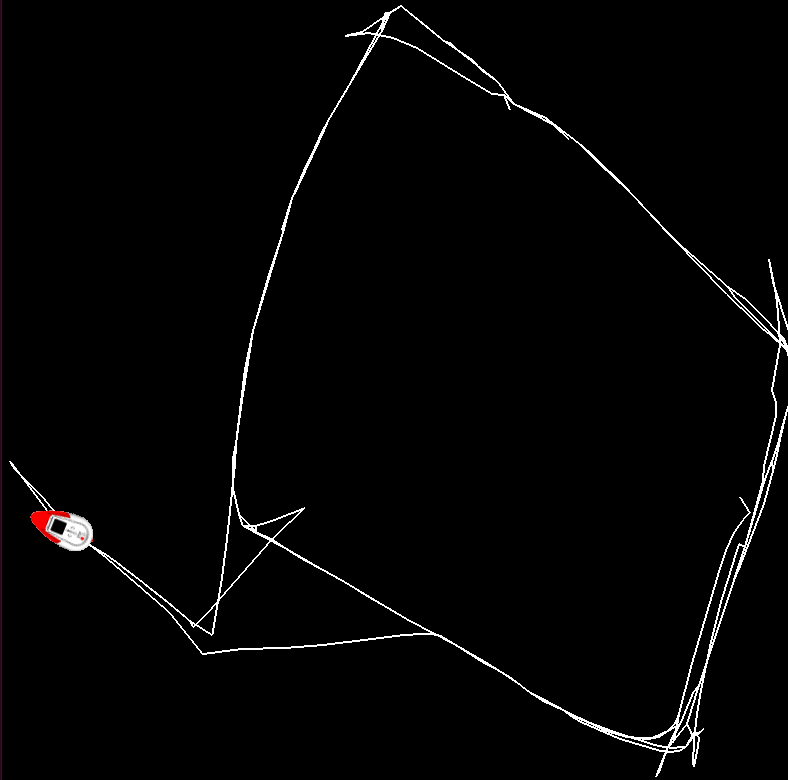
\includegraphics[height=0.3\textheight]{warehouse-1stStage.png}\label{fig:mapsWarehouse1st}}
    \hfill
    \subfloat[Both stages approaches]{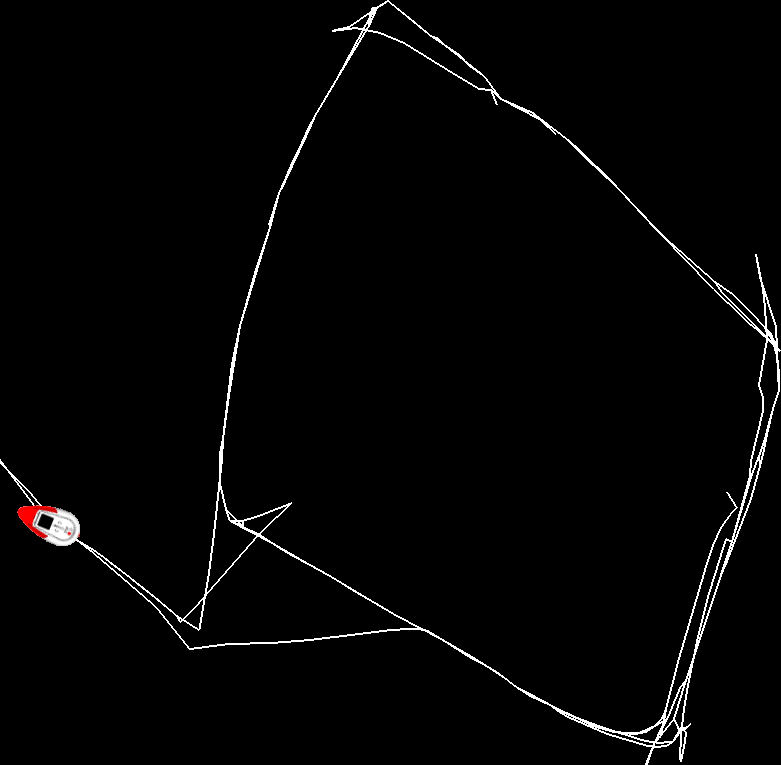
\includegraphics[height=0.3\textheight]{warehouse-bothStages.png}\label{fig:mapsWarehouseBot}}
    \\
    \subfloat[Original RatSLAM]{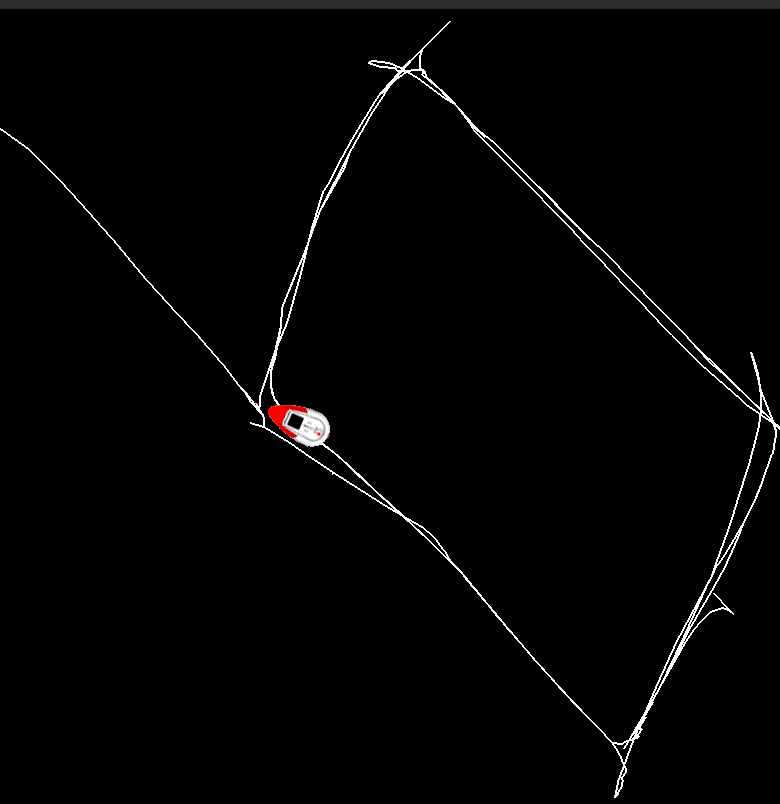
\includegraphics[height=0.3\textheight]{warehouse-ratslam.png}\label{fig:mapsWarehouseRat}}
    \hfill
    \subfloat[Exact trajectory]{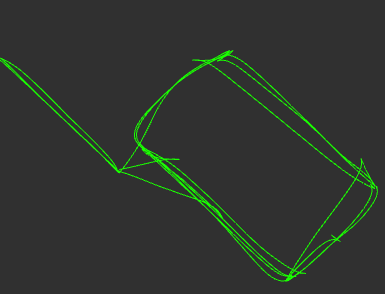
\includegraphics[height=0.3\textheight]{warehouse-exact.png}\label{fig:mapsWarehouseEx}}
    \caption{Generated experience maps in the warehouse environment}
    \label{fig:mapsWarehouse}
\end{figure}

\begin{figure}[!tbp]
    \centering
    \subfloat[1st Stage only approaches]{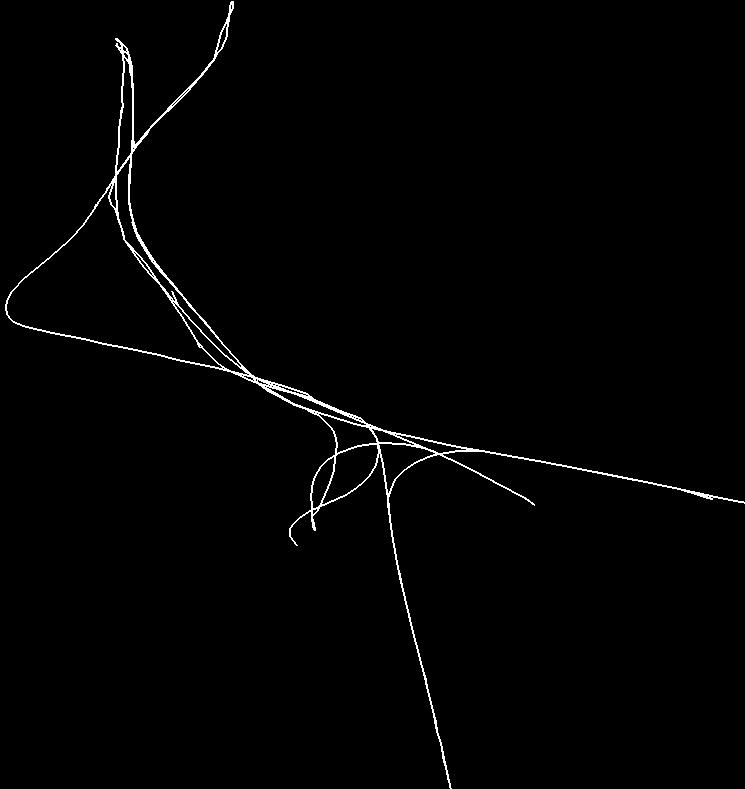
\includegraphics[height=0.3\textheight]{house-1stStage.png}\label{fig:mapsHouse1st}}
    \hfill
    \subfloat[Both stages approaches]{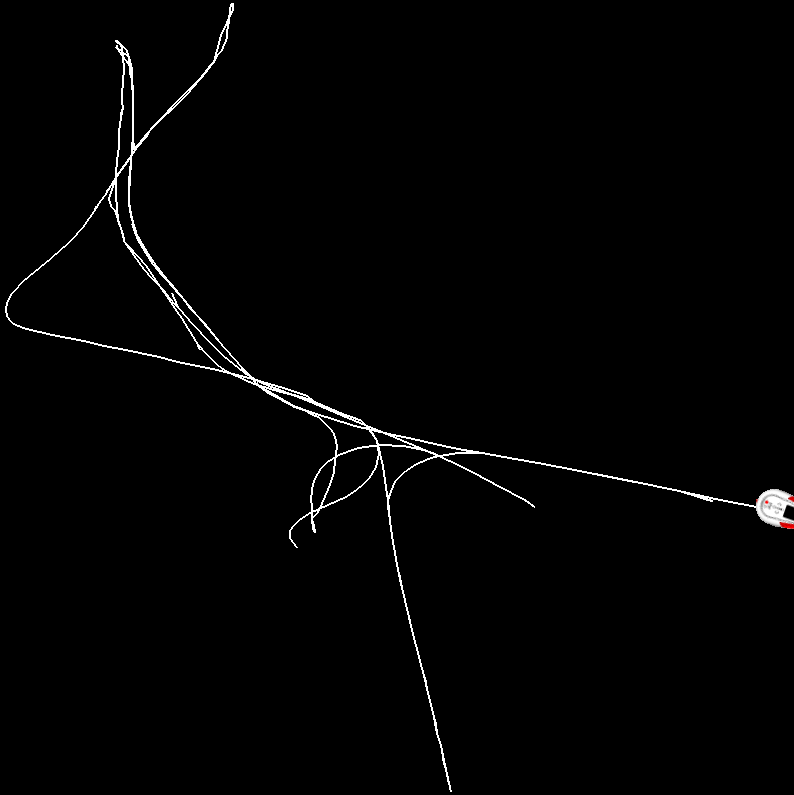
\includegraphics[height=0.3\textheight]{house-bothStages.png}\label{fig:mapsHouseBot}}
    \\
    \subfloat[Original RatSLAM]{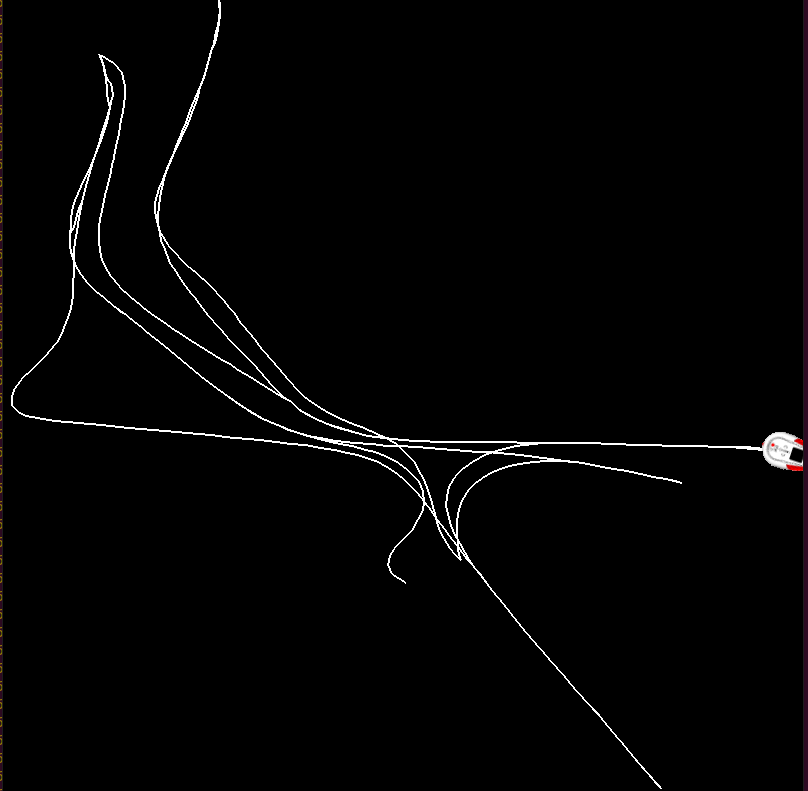
\includegraphics[height=0.3\textheight]{house-ratslam.png}\label{fig:mapsHouseRat}}
    \hfill
    \subfloat[Exact trajectory]{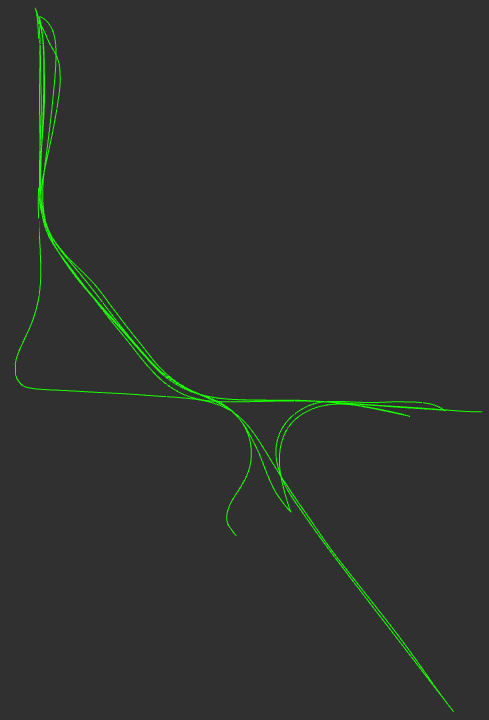
\includegraphics[height=0.3\textheight]{house-exact.png}\label{fig:mapsHouseEx}}
    \caption{Generated experience maps in the house environment}
    \label{fig:mapsHouse}
\end{figure}

\begin{figure}[!tbp]
    \centering
    \subfloat[1st Stage only approaches]{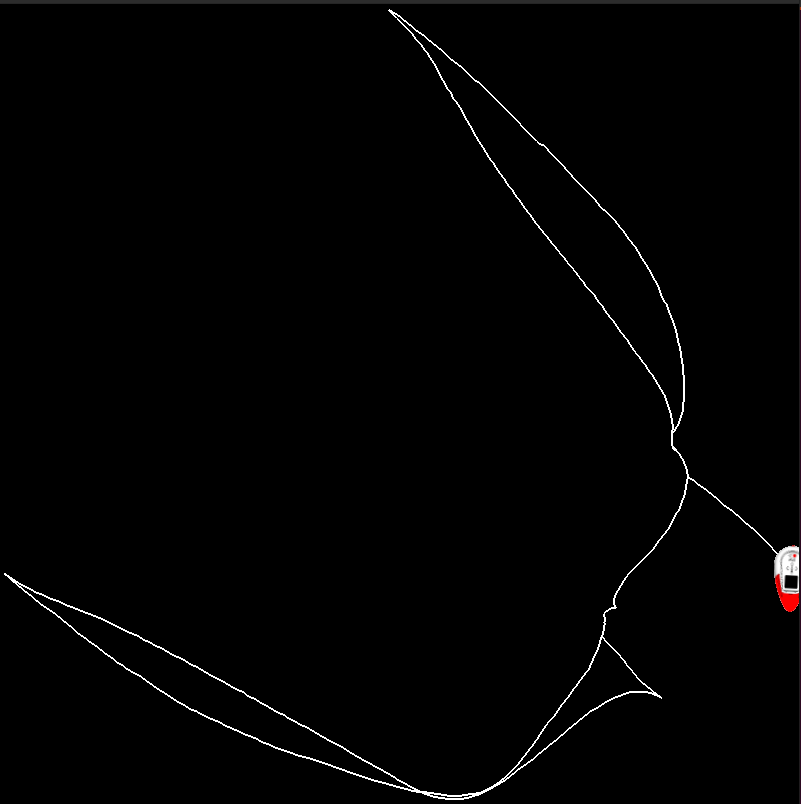
\includegraphics[height=0.3\textheight]{hospital-1stStage.png}\label{fig:mapsHospital1st}}
    \hfill
    \subfloat[Both stages approaches]{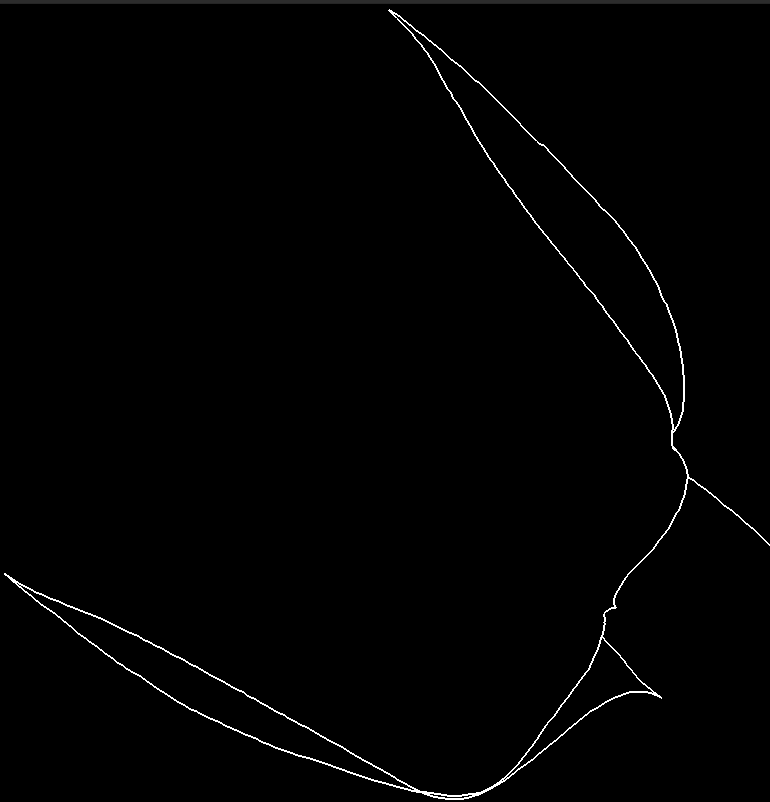
\includegraphics[height=0.3\textheight]{hospital-bothStages.png}\label{fig:mapsHospitalBot}}
    \\
    \subfloat[Original RatSLAM]{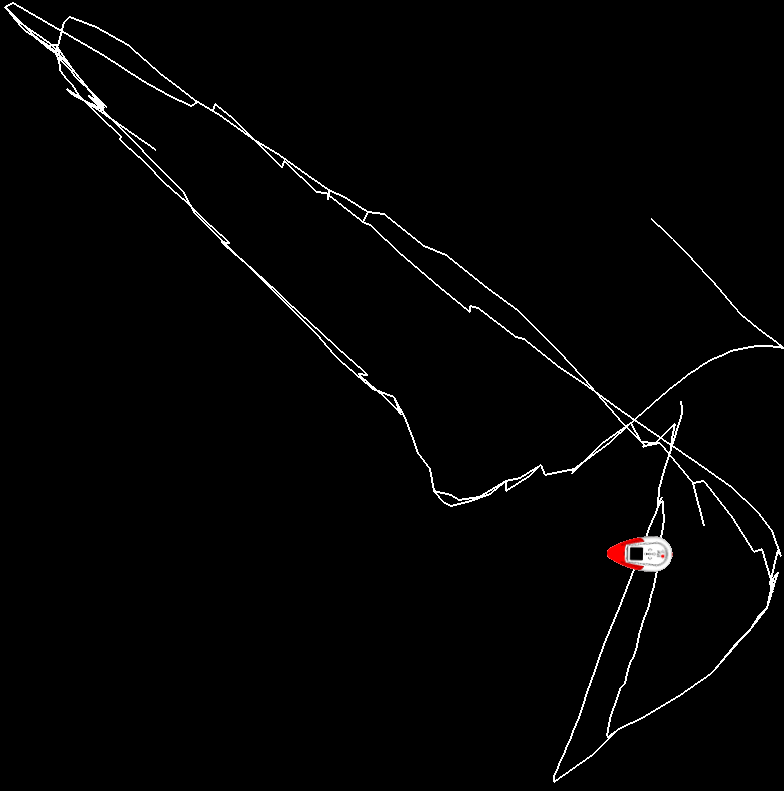
\includegraphics[height=0.3\textheight]{hospital-ratslam.png}\label{fig:mapsHospitalRat}}
    \hfill
    \subfloat[Exact trajectory]{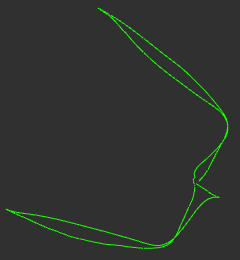
\includegraphics[height=0.3\textheight]{hospital-exact.png}\label{fig:mapsHospitalEx}}
    \caption{Generated experience maps in the hospital environment}
    \label{fig:mapsHospital}
\end{figure}

The figures \ref{fig:mapsWarehouse}, \ref{fig:mapsHouse}, and \ref{fig:mapsHospital} show the generated experience maps by every approach, including the original RatSLAM, together with the exact trajectory. The pictures clearly show that the results generated by the approaches with only the first stage and with both stages are almost identical. Even if the accuracy of the 2-stage approach was slightly better, the difference was too small to influence the results of the RatSLAM algorithm significantly. However, after comparing the generated maps with the exact trajectory, we can see that the results are satisfactory and that the suggested approaches are fully compatible with the RatSLAM algorithm.\par
Furthermore, the results from the hospital environment presented in figure \ref{fig:mapsHospital} clearly show that the suggested approaches can significantly outperform the original RatSLAM even in the generated trajectories. Because of the symmetry of the environment, the false evaluations of the visual scene recognition approach influenced the generated trajectory so significantly that it was entirely different from the exact one, and therefore, the original RatSLAM algorithm completely failed. However, the LiDAR sensors are considerably more precise in object distance estimation than a camera image, so the symmetry of the environment did not cause so many problems, and the generated results from the approaches suggested in this thesis were satisfactory.
